\chapter{Analysis}
\label{chap:analysis}

In this chapter, we analyze the \gls{sota} (see Part \ref{part:sota}) to define the scope of the \gls{poc} and add additional knowledgable details to project specifications as our initial understanding of the thesis subject increased. As a kickoff to research the \gls{sota} and for the analysis, in addition to peer consulting with our lab colleagues in the field of \gls{nlp}, we used curated lists e.g., awesome-nlp on Github \autocite{website:awesomenlp-github}. The knowledge accumulation started naturally to chain as we began to read papers mentioned in other papers.

\section{Rescoping and Motivations}
\label{analysis:rescoping}
Extrapolated from the \gls{sota} part \ref{part:sota}, we present in this section the process held to get to the final project scope based on the accumulated knowledge thru \gls{nlp} \gls{sota} exploration.

\subsection{Initial Project}
Our research initially started as a satellite to the \textit{AI-News} project (see Chapter \ref{intro:icosys}), which is currently using a Retrieval approach (see Chapter \ref{chatbot:retrieval}) combined with an intents and entities extraction, to return highly pondered recent articles from an elastic search in a Ruled-Based chatbot (see Chapter \ref{chatbot:rulebased}) format. The \textit{AI-News} project scoped our research indirectly toward finding solutions to bring \gls{qa} systems to the field of journalism; however, it early rescoped to open domain knowledge as the \gls{wikidata} \gls{kb} provides crowdsourced general knowledge. Additionally to the \gls{qa} scope, the specification implies \gls{nl} answers generation. We intended to build a \gls{qa} system to generate \gls{bleu} approved corpora based on the \gls{wikidata} \gls{kb}, then compare them to \gls{squad} benchmarking (see Chapter \ref{dataset:squad}), with the ultimate purpose to compare Pre-Trained Language Models such as BERT on your new dataset. As the starting point, we decided to bootstrap our project with \gls{sota} related papers filtered by code availability and reproducibility.

\subsection{Initial Ideas}
To achieve our initial project, we brainstormed the following ideas. Indeed, we expected to explore in detail the field of \gls{qa} evaluation in particular Oracle-based solutions, oracles are particularly meaningful in our context as we would use \gls{wikidata} as an oracle. Additionally, we planned to explore in more detail the effects of fine-tuning pre-trained language models such as \gls{bert}, with the intent to create a challenging dataset. Based on a finite state grammar, our evaluation would initially generate a set of 100'000 \gls{wikidata} \gls{spo}-based questions and using word-embedding similarity feature to paraphrase those questions to increase complexity. We even discuss an additional feature to generate \gls{qa} multi-turns conversations (see Chapter \ref{chatbot:context}) by self-training a model with an \gls{al} approach.


\subsection{Second Brainstorming Iteration}
As research progressed, we took the party that we did not want to be just another benchmarking system for \gls{qa} systems, similarly to our initial decision not to become an nth fine-tuned pre-trained language model. As a result, our second brainstorming iteration brought quite a new scope to the project. Indeed, we focused mainly on a \gls{mh} multi-turns conversations approach, by aiming at building an interactive and proactive reversed Akinator-like \autocite{website:akinator} \gls{qa} system. The system would use a \say{child} learning approach as the model itself starts with no knowledge, and incrementally learns new knowledge by interacting with users. The goal is to teach the model to retrieve information from a \gls{kb} by itself. The game consists of a randomly selected \gls{wikidata} entity as the answer, and the user is requested to help, via a gamified conversational interaction, the bot to build a path in \gls{wikidata}, as it asks questions to the user. The proactive ability would a generative approach to scenario-based chatbot like HelloJam \autocite{website:hellojam}, which uses intermediary steps as a proactive approach. As a training bootstrap, we initially planned to build a conversational simulator using multi-hop datasets such as ConvQuestions, \gls{squad}, or \gls{quac}.


\section{Third Brainstorming Iteration}
Quickly, the previous brainstorming iteration raised problems such as the truth user interest for such games and the bias induced by genuine or intentional human errors, without mentioning the pre-processing needed to build a meaningful training dataset, but we kept some ideas. We believed that the \gls{mh} multi-turns conversations are an essential feature to our work, combined with the interactive and proactive approach between the bot and the user, which is a particularly exciting application in the \gls{nlp} field. We then suggested a new shift in the project scope to build \gls{nl} \gls{qa} chatbot allowing the user to interact with the conversation and the knowledge in a meaningful manner. The goal is to provide the user the ability to check returned answers with facts and correct them on the fly if needed. Additionally, we wanted to add a multi-model approach to handle virtual personalities as a flavor of personalization to the user.


\subsection{Final Brainstorming Iteration}
The project scope shifted one last time. We noticed that the applications in the field of \gls{qa}, and \gls{generative} chatbot are extensive, and it appeared that it is possible to find a paper already mentioning, even lightly, what we believed original ideas. As a contradiction, we decided at aiming directly at the roots of \gls{qa} and \gls{generative} systems as a whole. To do so, we kept the multi-hops reasoning, multi-turn conversations, and the \gls{wikidata} \gls{kb} as constraints to the project. Indeed, we did not want to be just another \gls{transformer} related project trying to define the new baseline. Our resources at disposal were limited, and we wanted to take a new approach by exploring an original technique for \gls{qa}, in particular, Sub-Knowledge Graphs. To achieve our latest project, we examined existing \gls{sota} systems providing, in addition to the paper, a runnable code to get started. We initially aimed at incrementally improve the original work to impact the \gls{nlp} field. Our first step was to reproduce the results; then, the second step was to retrain and provide additional value to the original work. And finally, adapt the initial project to the News field with few tweaks. 

\section{Question-Answering Systems Choices}
Based on the \gls{sota} (see Part \ref{part:sota}) and the previous rescoping section \ref{analysis:rescoping}, we aim at building a \gls{qa} \gls{mh} and multi-turn converstational chatbot using sub-graphs from \gls{wikidata}. We found a unique direct competitor to our work, and we are using its baselines and nested baselines to compare our work.

\subsection{Competitors}
We initially explored \gls{qa} system using the \gls{wikidata} \gls{kb} by default, and providing the must-have features defined in the project scope, our research revealed a unique candidate and two related candidates as they define the baseline of our main candidate.

\paragraph{CONVEX}
As our direct competitor, CONVEX \autocite{paper:convex} (see Chapter \ref{eval:convex}) extracts sub-graph from \gls{wikidata} \gls{kb}. It employs the sub-graphs as context holders and uses them to answer context-related questions via a frontier algorithm. It finally extends the context-graph with the new answers, making the graph more precise at answering detailed questions.

\paragraph{qAnswer and Platypus}
Both \gls{qa} systems are using a template-based model (see Chapters \ref{eval:qanswer} and \ref{eval:platypus}), and are defined as baseline in our main candidate and they are designed to for \gls{wikidata} queries. Note that they are \gls{sh} and trained on the SimpleQuestions dataset, which we also plan to use as a fair evaluation.


\subsection{Datasets}
Our initial predetermined dataset was \gls{squad} due to its popularity and its public leaderboard, as it would have been a pleasant additional comparison to our work. However, \gls{squad} is designed to answer fact-based questions with a span extracted from the given context paragraph, often implying a mismatch with fact entities such as in the \gls{wikidata} \gls{kb}. It is also a reason for CONVEX to not evaluate on this dataset, similarly to qAnswer and Playtypus. Finally, in the scope of the project, we did not plan to adapt the \gls{squad} dataset for \gls{wikidata}-based \gls{qa} systems.

\paragraph{ConvQuestions}
As descried in Evaluation Chapter (see \ref{eval:convex}), CONVEX \autocite{paper:convex} is design to use the ConvQuestions dataset (see Chapter \ref{dataset:convquestions}), which is a multi-turn conversations and \gls{mh} \gls{qa} crowdsourced dataset. CONVEX uses also this dataset with its baselines providing an initial evaluation for all three competitors.

\paragraph{SimpleQuestions}
As presented in the Dataset Chapter (see \ref{dataset:simplequestions}), SimpleQuestions has a \gls{wikidata} \gls{kb} adaptation provided by Playtpus authors \autocite{paper:InProceedingsPellissier-Tanon.P-TD-d-ACM-S_18}. This dataset will be used to benchmark our system in addition to all three competitors, as a fair approach to evaluate \gls{sh} systems on \gls{sh} design datasets.

\subsection{Benchmarking}
To measure and compare our work, we will set up two benchmarks. The first benchmark will evaluate the \gls{sh} capabilities of each competitor on the \gls{wikidata} adapted SimpleQuestions dataset. The second benchmark is focusing on the \gls{mh} and multi-turn conversations capabilities from each competitor. As qAnswer and Platypus are not designed for multi-turn conversations, we will extend them with CONVEX and our work during the multi-turn task, as both projects can work on top of other algorithms (see the next Chapter \ref{chap:graphqa}).



\section{Texts Generation Choices}
We plan to used two \gls{sota} pre-trained \gls{lm} in there vanillia large format, \gls{bert} \autocite{paper:devlin-etal-2019-bert} and \gls{gpt2} \autocite{papers:gpt2}, for our text generation \gls{nlp} task. \gls{bert} will be used as a text filler for the SPOs paths extracted complementary to the answer from the \gls{wikidata} Sub-Knowledge Graphs. \gls{gpt2} will be used as a complementary facts generator to the answer.

\paragraph{Evaluation}
We consider \textit{Google's} dataset (see Chapter \ref{dataset:googlenatural}) as promising; however, we did not plan to evaluate our generated \gls{nl} answers on this dataset as the project planning is too tight to include this protocol. We instead, we will assess the dialogues generated manually. An evaluation idea would be to run a campaign with 10 to 20 users evaluating 10 to 20 questions, using the evaluation tags: \say{Good}, \say{Neutral}, or \say{Bad}. However, this dataset is worth considering for future extended work. 

\section{Final Project Scope}
GraphQA, as we name it, is a \gls{qa} Sub-Knowledge Graphs chatbot using  the \gls{wikidata} \gls{kb} database. It extracts answers to questions from a complete \gls{linked-data} database by extracting small portions of the main database and manipulates it as a graph. The graph manipulation implies context holding, extension, and refining. Initially, based on CONVEX, we plan to improve their \gls{ir}-based answering to the first answer, as it is their bottleneck, which is particularly sensitive as it defines a successful anchor to a conversation-driven \gls{qa}. We wish to also explore sub-graph capabilities with temporally depend contexts, and their overall performances. Additionally, \gls{nl} capabilities must be present by combining two complementary pre-trained language models.

\subsubsection{Expected Features}
We define below the features we expect to be present in GraphQA as a \gls{mh} Conversational \gls{qa} Chatbot.

\begin{itemize}
    \setlength\itemsep{0em}
    \item Extract question keywords.
    \item Extract a question-related Sub-Knowledge Graph.
    \item Compute the answer from the Sub-Knowledge Graph.
    \item Extract an SPO Tuple meaningful to the question.
    \item Prune the Sub-Knowledge Graph of context meaningless elements
    \item Generate a \gls{nl} answer from the SPO Tuple.
    \item Extend the \gls{nl} generate an answer with additional facts.
    \item Extend the Sub-Knowledge Graph with new questions.
\end{itemize}


\subsubsection{Nice to have}
As we do not expect to have the time to add additional features to the primary features described in the above subsection. We are mentioning some features that we would like to see in the project one day. Note that \gls{kb} databases are by design only as good as the data the relations they hold, which is limited also by the employed schemas, implying if the reasoning information such as quantities were not manually referenced into the database, the answer is impossible to retrieve.

\begin{itemize}
    \setlength\itemsep{0em}
    \item Give the ability to merge pre-generated sub-graphs.
    \item Use of multiple modules to manage different processes.
    \item Include reasoning modules such as inductive logic or quantification.
    \item Provide an auto-correct tool to users.
    \item Provide an auto-complete tool to users.
    \item Provide a paraphrasing tool to generated answers.
    \item Use the multilingual \gls{wikidata}'s propriety paraphrase into a translation.
    \item Use \gls{wikidata}'s multi-properties to paraphrase questions and answers.
    \item Handle pre-built sub-graphs for particular subjects such as Articles, Countries, Movies, or Famous People
    \item Track users custom sub-graphs to track the overall context.
    \item Use consensus-based modules to complementarily provide the best answers.
    \item Show visually to users their sub-graph generation
    \item Provide on-the-fly tools to modify sub-graphs.
\end{itemize}



\section{CONVEX Q0 Solutions}
As mentioned in previous sections and represented on the Figure \ref{fig:fig_high_level_convex_architecture_analysis}, CONVEX \autocite{paper:convex} has an issue with the first answer. The issue has been briefly explored and confirmed in the CONVEX paper. Indeed, for a0 (the initial answer), CONVEX uses a proprietary \gls{ner} system, TAGME \autocite{paper:CIKM-2010-FerraginaS}, as its \gls{wikidata} entities identify system. Then places into an empty a subgraph returned entities with their relation extracted from the \gls{wikidata} \gls{kb}. This process is solely relying on a TAGME to answer the initial question, which are often interpreted as lucky guesses. As one of our main contributions, we want to fix this issue, and to do so, we propose five different solutions, including a naive one. 

\begin{figure}[H]
    \centering
    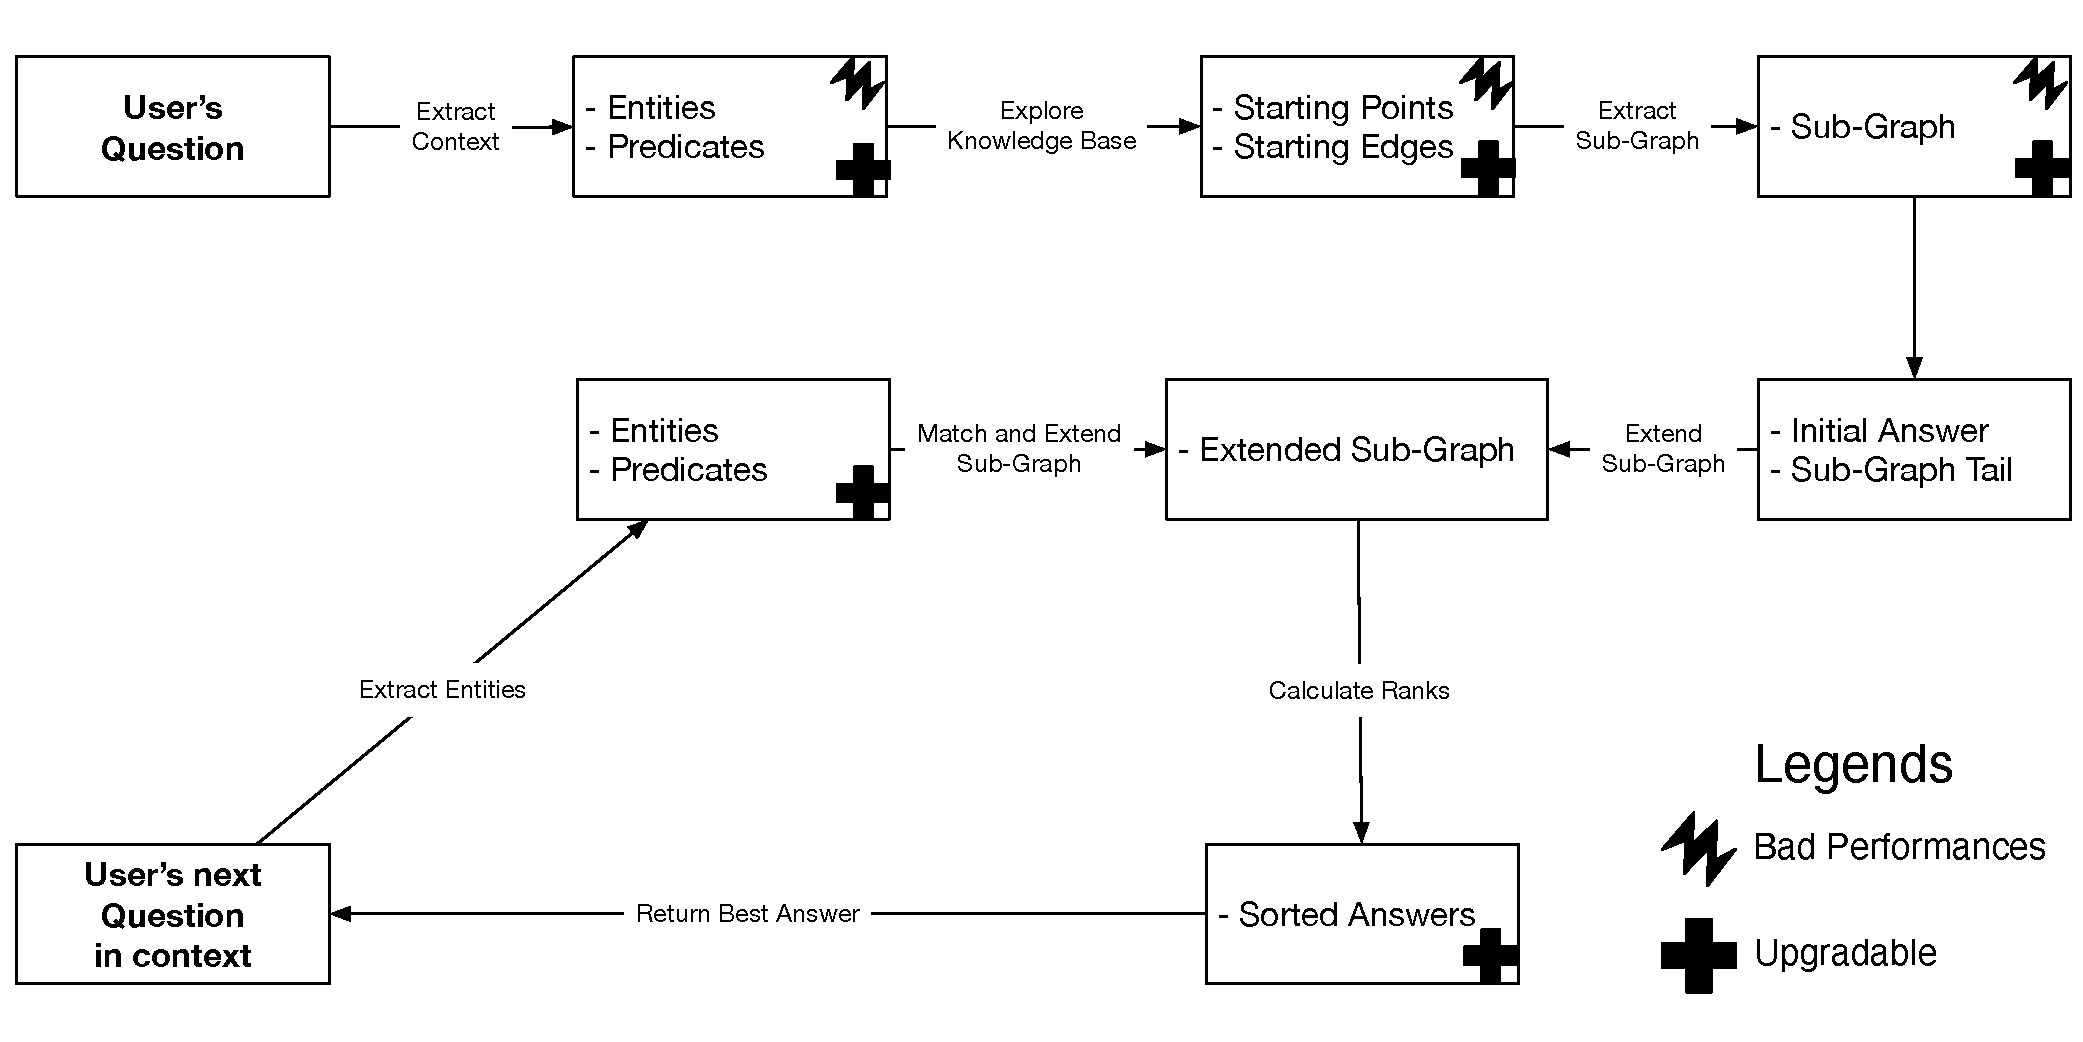
\includegraphics[width=\textwidth,keepaspectratio=true]{fig_high_level_convex_architecture_analysis}
    \caption{Illustrative representation of the high level CONVEX architecture. the diagram includes the identified part having bad performances, and shows the upgradable components.}
    \label{fig:fig_high_level_convex_architecture_analysis}
\end{figure}

\subsection{0th Solution: Naive Approach}
Our naive approach is to use text summarization to extract relevant information and build the initial sub-knowledge graph by matching the entities present in the \gls{wikidata} \gls{kb}. It is indeed not an impressive approach by at least we have control over the extracted data, and we can study the related induced behaviors, then tune the system with additional models.

\subsection{1st Solution: BiDAF++}
\label{analysis:bidaf}
The BiDAF++ model, presented with \gls{quac} \autocite{paper:journals/corr/abs-1808-07036}, is based on BiDAF \autocite{paper:journals/corr/SeoKFH16} augmented with self-attention \autocite{paper:journals/corr/abs-1710-10723} and ELMo \autocite{paper:journals/corr/abs-1802-05365}, and particularly used as non-\gls{transformer} baseline on multiple \gls{qa} datasets. We could explore training on multiple dataset such as Google's Natural Questions Corpus \autocite{paper:google-natural-questions}, ConvQuestions \autocite{paper:convex}, CoQA \autocite{paper:journals/corr/abs-1808-07042} and NewsQA \autocite{paper:journals/corr/TrischlerWYHSBS16}. The model would provide us the answers to the questions, and we would build the initial sub-graph based on the matched entities id found in the question and the entity found as the answer.

\subsection{2nd Solution: Multi-task learning}
Multi-task learning for large scale \gls{kb} \autocite{paper:2019arXiv191005069S} is by design handling the conversational \gls{qa} format, making it particularly appealing to our project. The techniques model trained to parse questions and point them into the \gls{kb} via pointers, which avoids the propagation of errors and simultaneously exploits the pointer property to share the linked information.

\subsection{3rd Solution: Knowledge Graph Embedding}
Knowledge Graph Embedding \autocite{paper:2019arXiv191102168W} is model trained to locate entities (subject) and predicates individually in a \gls{kg} and then predict the tail (object). However, this technique, as described by the authors, works only for simple questions, which conflicts with our \gls{mh} constraint, implying to extend the model capabilities to \gls{mh} handling. 

\subsection{4th Solution: Fine-tuned Pre-trained Language Model}
Even if we do not expect to use this solution, it is still worth mentioning. Indeed, the final solution would be to fine-tune a transformer-based model on multiple \gls{qa} datasets similarity mentioned in the 1st solution above (see Subsection, \ref{analysis:bidaf}).


\subsection{Our representation in the Chatbot Cartography}
To conclude this chapter, we updated the chatbots cartography as defined in the chatbot state-of-the-art chapter (see \ref{chatbot:cartography}) to illustrate our position. (See Figure \ref{fig:fig_chatbot_cartography_graphqa})

\begin{figure}[H]
    \centering
    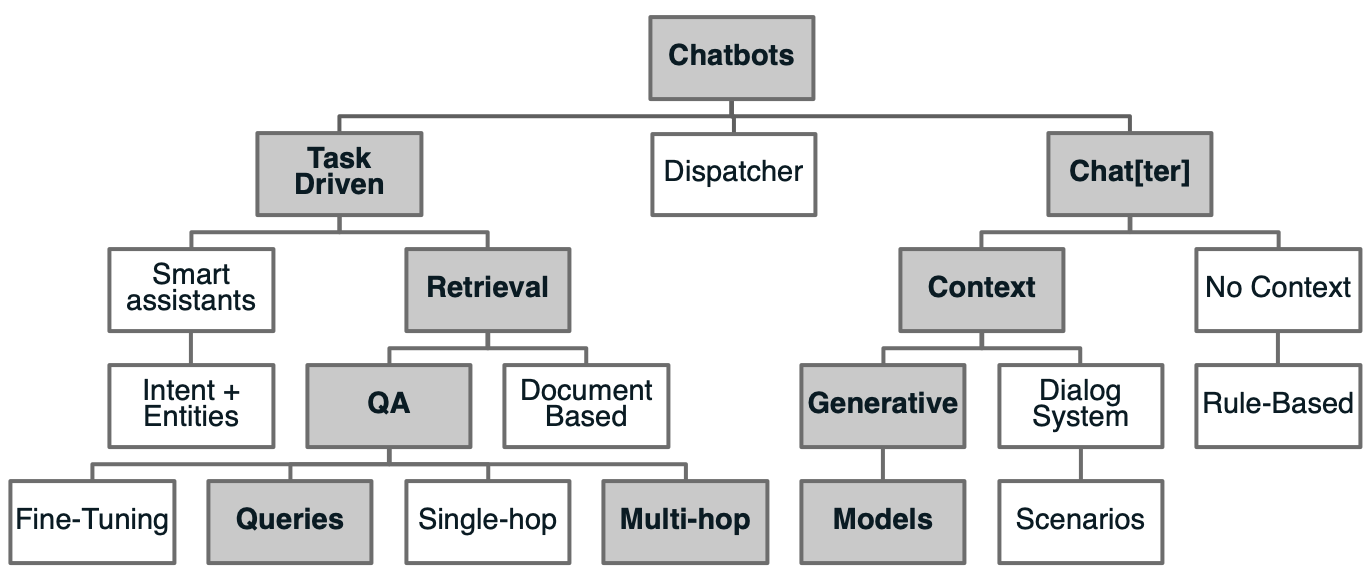
\includegraphics[width=\textwidth,keepaspectratio=true]{fig_chatbot_cartography_graphqa}
    \caption{Represents GraphQA's positions in the chatbots cartography as defined in the chatbot state-of-the-art chapter.}
    \label{fig:fig_chatbot_cartography_graphqa}
\end{figure}

